\chapter{Architectual Diagram}
This system has a data-flow architecture (see Figure~\ref{fig:architectualDiagram}), starts from "Headset" and move clock-wise to "Audio". The reason of choosing this architecture is because there are constant inputs received by the system, and the inputs in general goes through the same route within the system. The data-flow architecture also has build in concurrency, which can speeds up the process, especially the platform of the product is embedded.
\begin{figure}
	\label{fig:architectualDiagram}
	\centering
    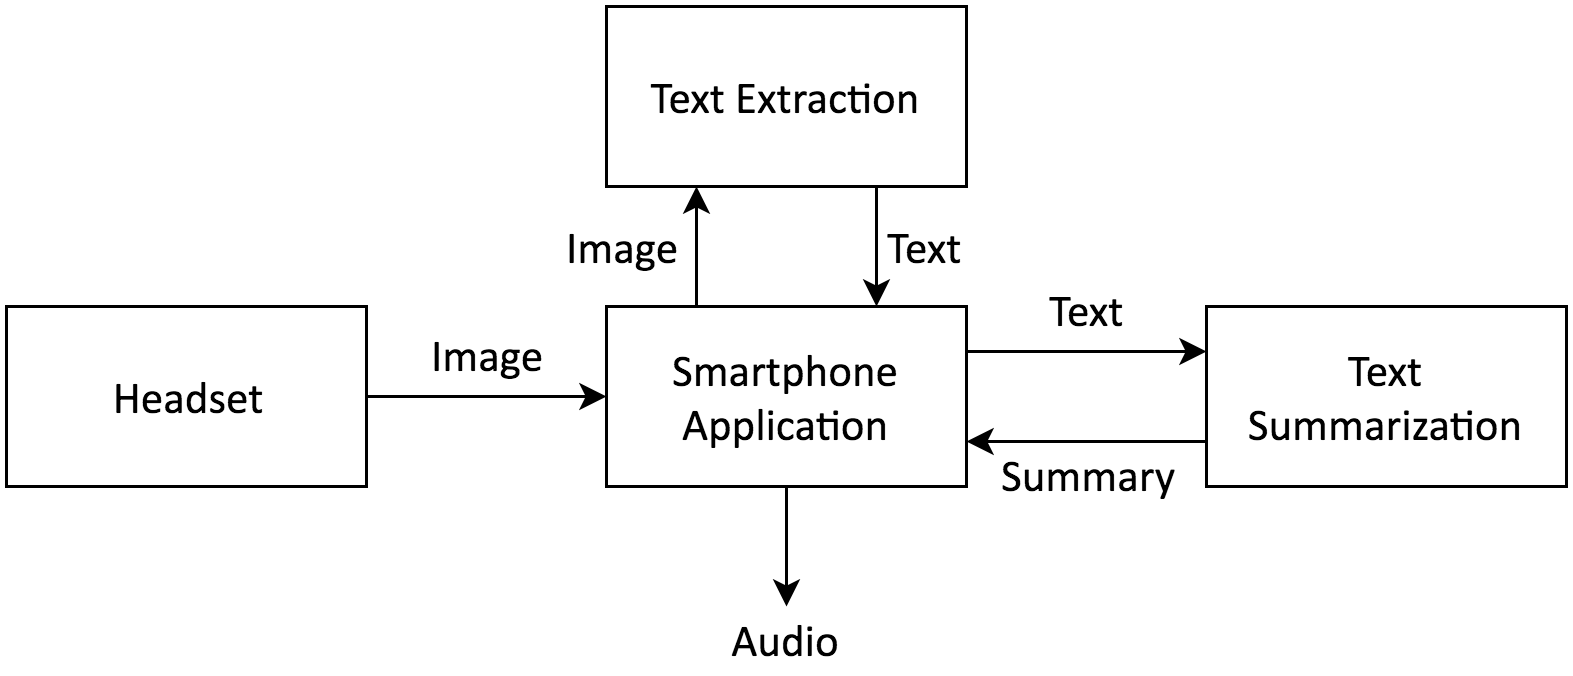
\includegraphics[scale = 0.2]{ArchitectureDiagram.png}
    
    \caption{Architectual Diagram}
\end{figure}